\section{Projektplanung}
\label{projektplanung}

In diesem Kapitel werden das Projektmanagement und der Projektplan der Teamarbeit aufgezeigt.
Es wird dieselbe Projektmanagementmethode verwendet wie in \acrfull{pren1}: Es wird Scrum auf das Projekt angepasst. Synchronisationsmeetings finden wöchentlich statt, es wird inkrementell gearbeitet und am Ende der timeboxed Sprints gibt es ein funktionierendes Produkt. Zu Ende von jedem Sprint wird geprüft, ob die Sprintziele erreicht wurden.\cite{wikipedia-scrum}

Ebenso sind der Datenaustausch, die Kostensammlung und die verwendeten Tools gleich. Nach wie vor wird Microsoft Teams als Tool verwendet, um Informationen zu speichern und auszutauschen und es wird wieder das Scrumboard von Teams verwendet.

\subsection{Organigramm}

Die Teamzusammenstellung hat sich leicht geändert, da ein Student das Team nach \acrshort{pren1} verliess und ein neuer Student das Team betrat. Die zugewiesenen Rollen sind nach wie vor dieselben, wie in \acrshort{pren1}.

TODO BILD

\subsection{Releaseplan}

Die Arbeitszeit wurde in 4 Sprints aufgeteilt, wobei die ersten 3 Sprints 4 Wochen dauern und der letzte Sprint 3. Die Daten der Sprints und der Meilensteine sind auf folgender Grafik \ref{fig:project-plan} sichtbar.


\begin{figure}[H]
\centering
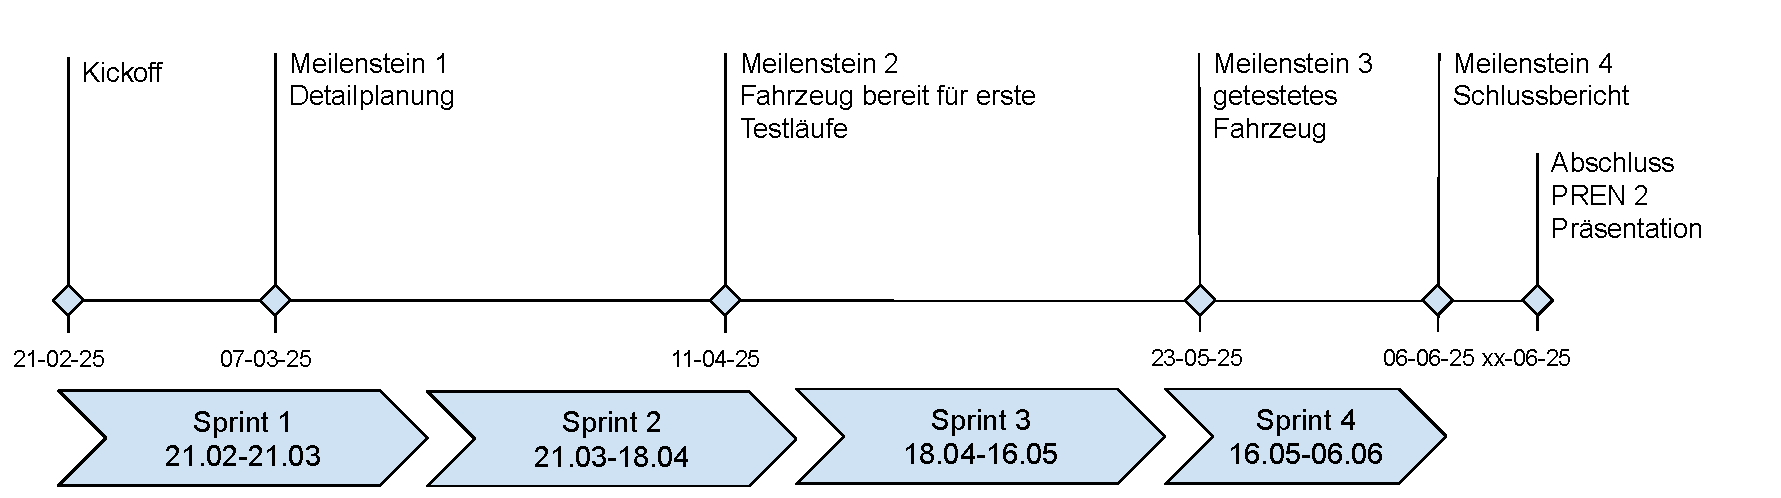
\includegraphics[width=\textwidth]{assets/projektmanagement/projektplan.pdf}
\caption{Projektplan}
\label{fig:project-plan}
\end{figure}

\subsection{Backlog}

Der Backlog dient als zentrales Planungselement.
Nach dem Abschliessen eines Sprints wird ein Ausblick auf den nächsten Sprint durchgeführt, um allfällige Anpassungen an dessen Sprintbacklog vorzunehmen. Ebenfalls wird zu Ende eines Sprints ein Controlling durchgeführt.

Der folgende Plan in Tabelle \ref{table:release-plan} zeigt die einzelnen Teilfunktionen des Roboters mit verfeinerten User Stories. Die Epics wurden priorisiert und Sprints zugeordnet und die Aufwänder der User Stories wurden in Personentagen (8 Stunden) geschätzt und ebenfalls den einzelnen Disziplinen zugeordnet. Diese Zuordnung zu den Disziplinen dient der Übersicht und kann abweichen.
Die Schätzungen der User Stories beinhalten die Dokumentation und das Testen der Arbeiten. Die Epics sind aufeinander aufbauend. Es kann parallel daran gearbeitet werden, aber um die einzelnen Produkte am Roboter zusammenfügen zu Können, müssen oft bestimmte User Stories zuvor bereits abgeschlossen werden sein. Diese Abhängigkeiten sind in den einzelnen Sprints nachfolgend beschrieben. Die Priorisierung wurde zum einen nach diesem aufbauenden Prinzip durchgeführt, als auch danach, welche Stories das höchste Risiko aufweisen. Diese Stories wurden höher priorisiert, damit mehr Zeit für eine allfällige Problembehebung vorhanden ist.
Die Farben der einzelnen Epics dienen lediglich zu einem besseren Überblick.

TODO: UGLY


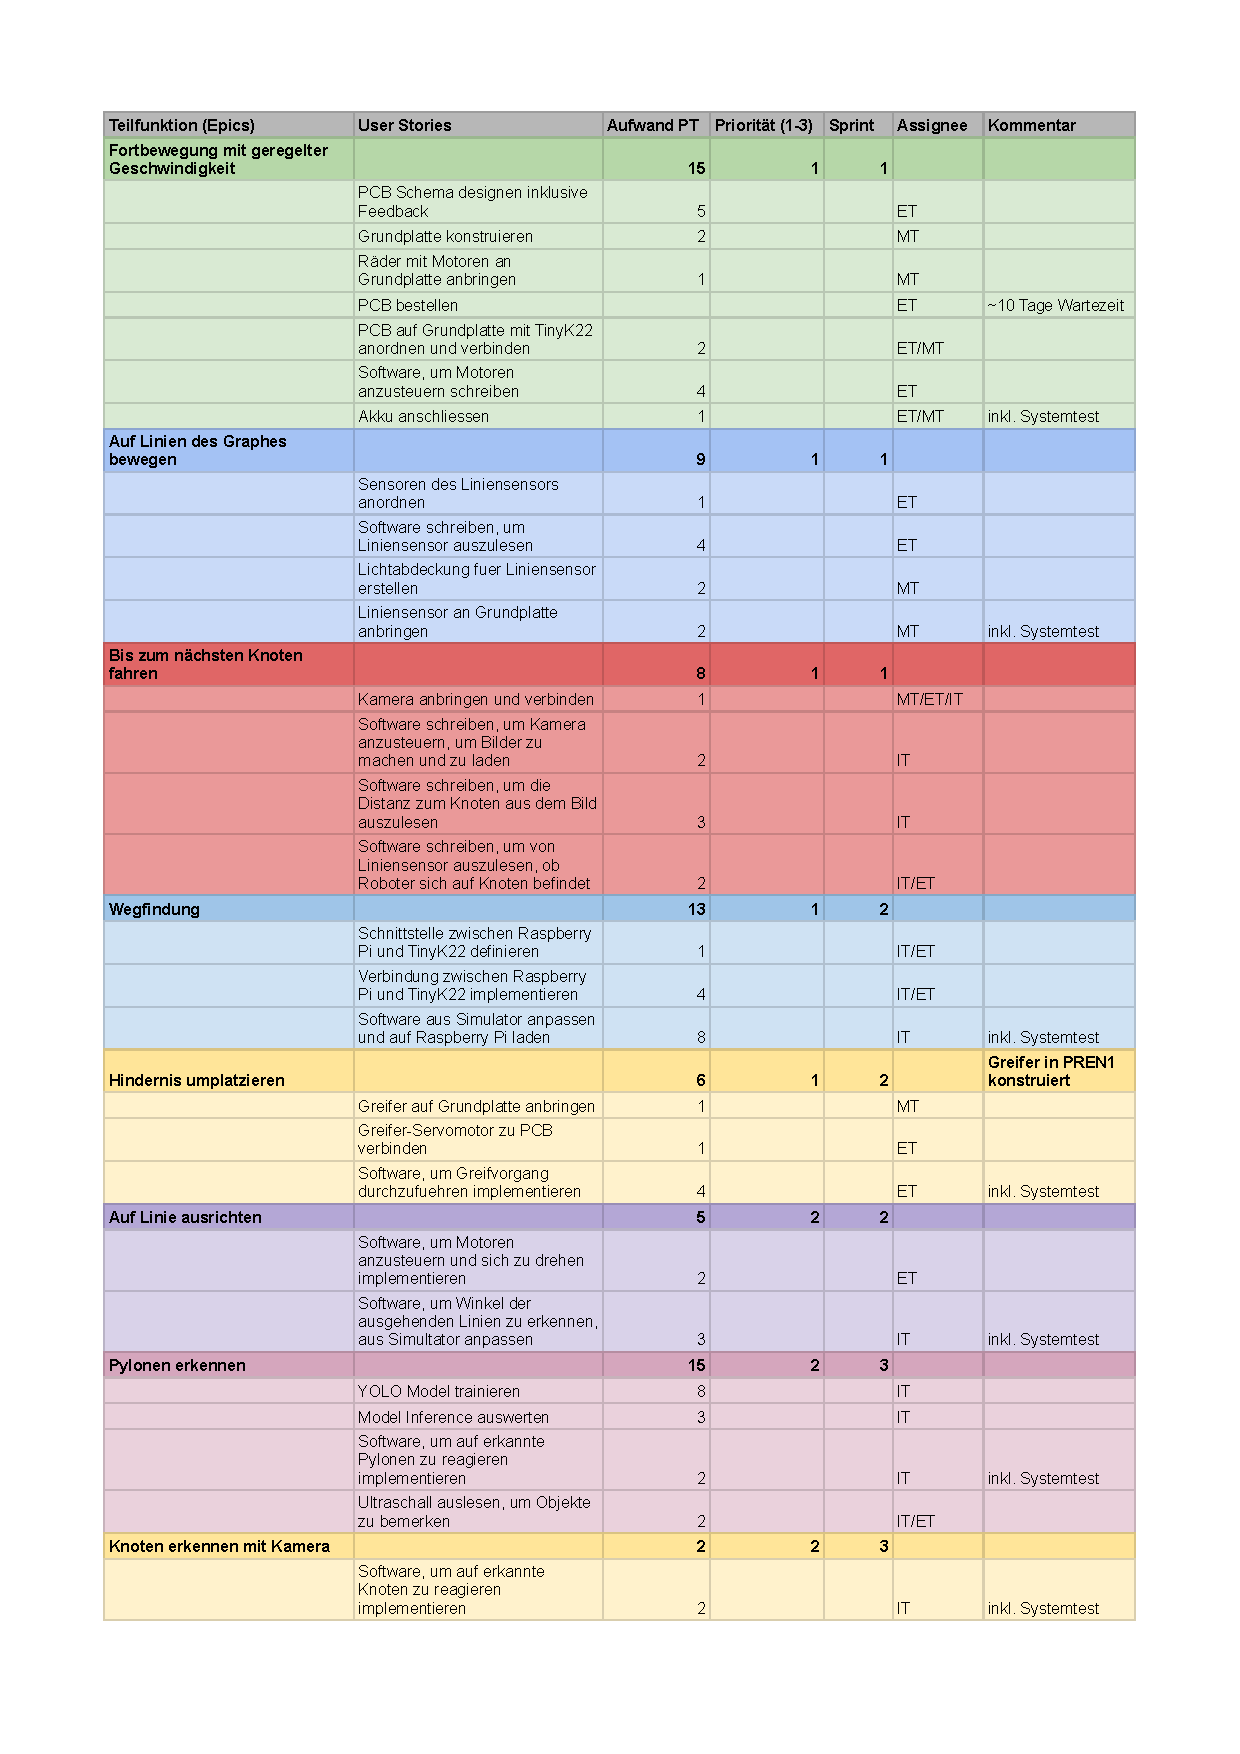
\includepdf[pages=-]{assets/projektmanagement/releaseplan-alle-sprints.pdf}
\begin{table}[H]
\centering
% 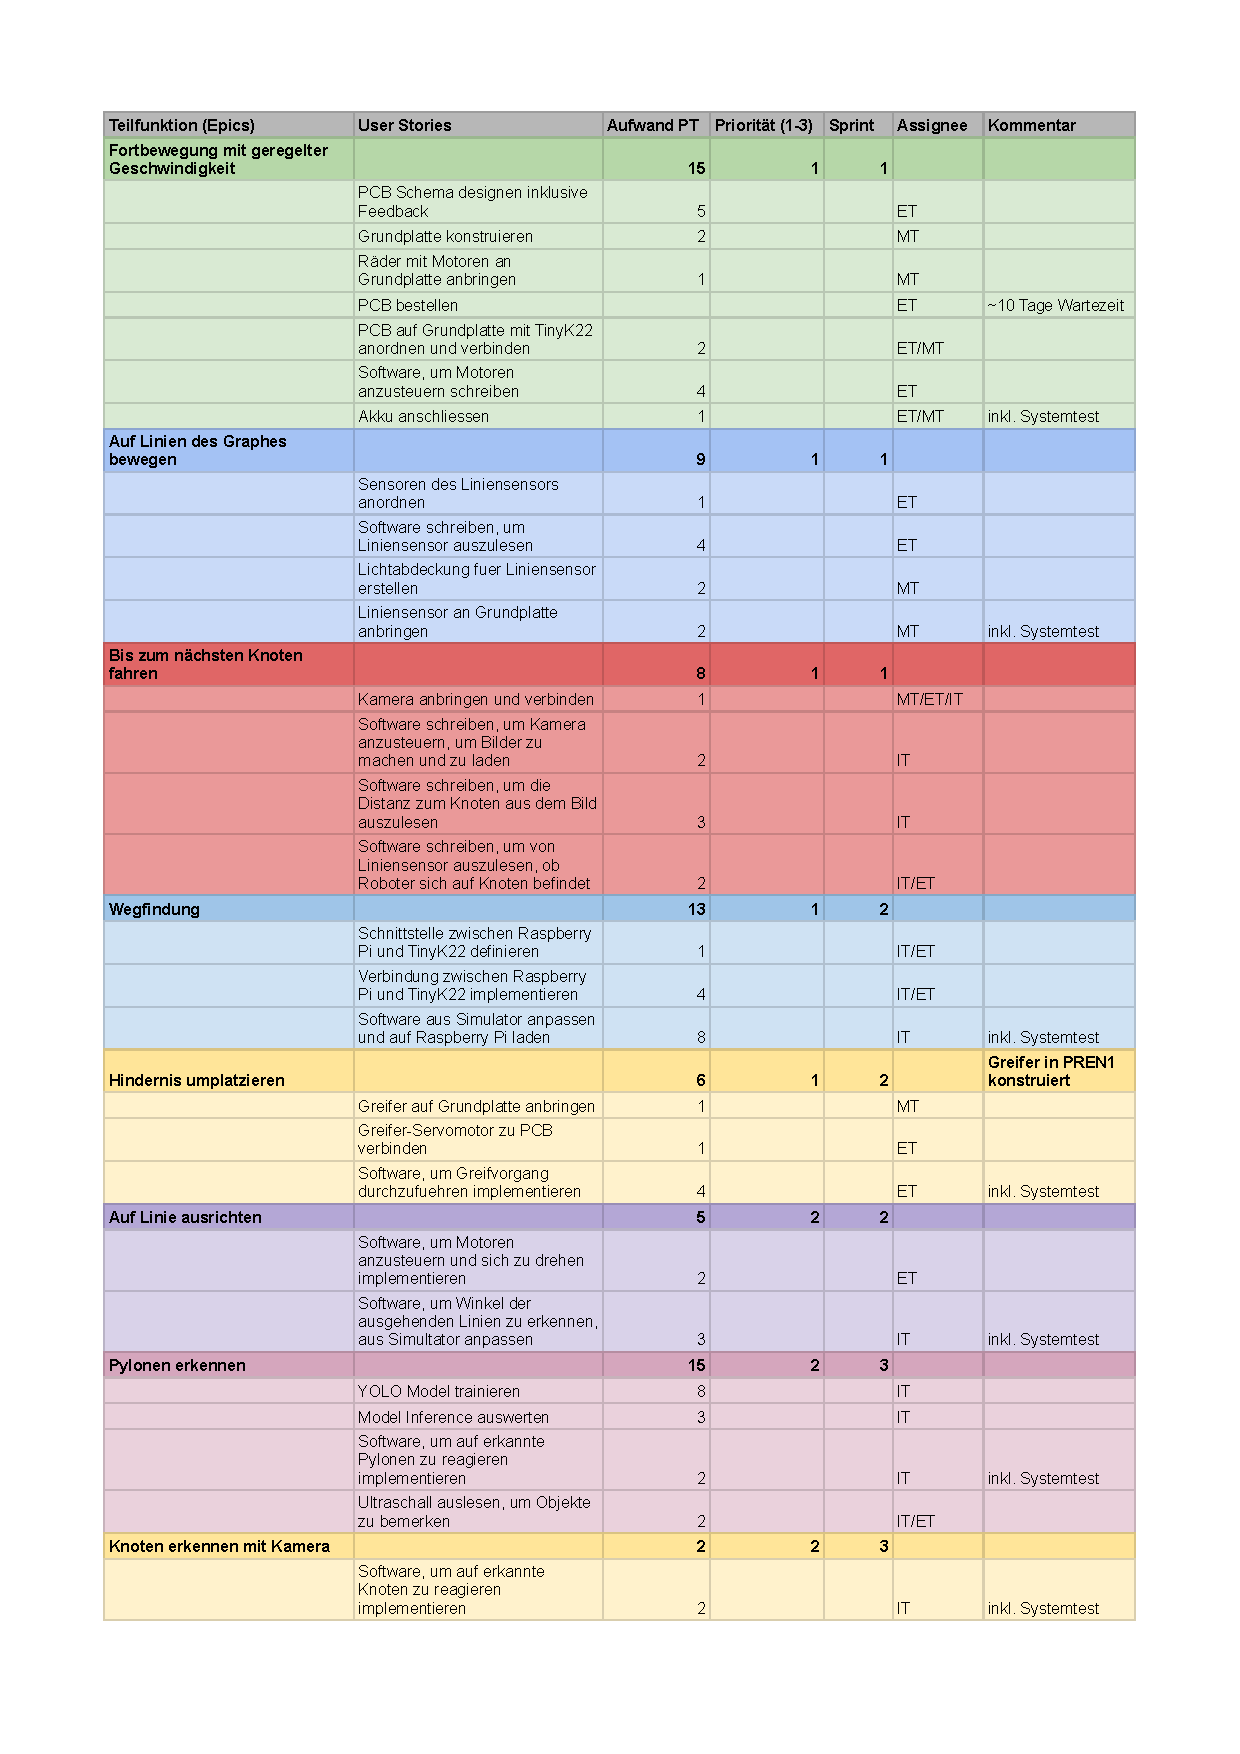
\includegraphics[width=\textwidth]{assets/projektmanagement/releaseplan-alle-sprints.pdf}
\caption{Releaseplan}
\label{table:release-plan}
\end{table}


\subsection{Sprintplanung}

In den folgenden Kapiteln wurden für jeden Sprint Sprintziele und ein Sprintbacklog definiert. Dieser ergibt sich aus dem Releaseplan. Darin wird der geschätzte Aufwand mit dem tatsächlichen Aufwand verglichen. Ebenfalls wird angegeben, falls eine User Story nicht fertiggestellt wurden konnte in dem geplanten Sprint.

\subsection{Sprint 1}

\textbf{Sprintziele:}
\begin{itemize}
    \item Der Roboter soll von Software gesteuert geradeaus fahren können.
    \item Der Roboter soll von Software gesteuert, einer Linie folgen können.
    \item Der Roboter soll von Software gesteuert, von einem Knoten aus zu einem Nachbars Knoten, der unter 2 Meter entfernt ist, fahren können.
\end{itemize}

\textbf{Sprintbacklog:} Der Sprintbacklog von Sprint 1 ist in Tabelle 
\ref{table:sprint1-backlog} 
dargestellt.

\begin{table}[H]
\centering
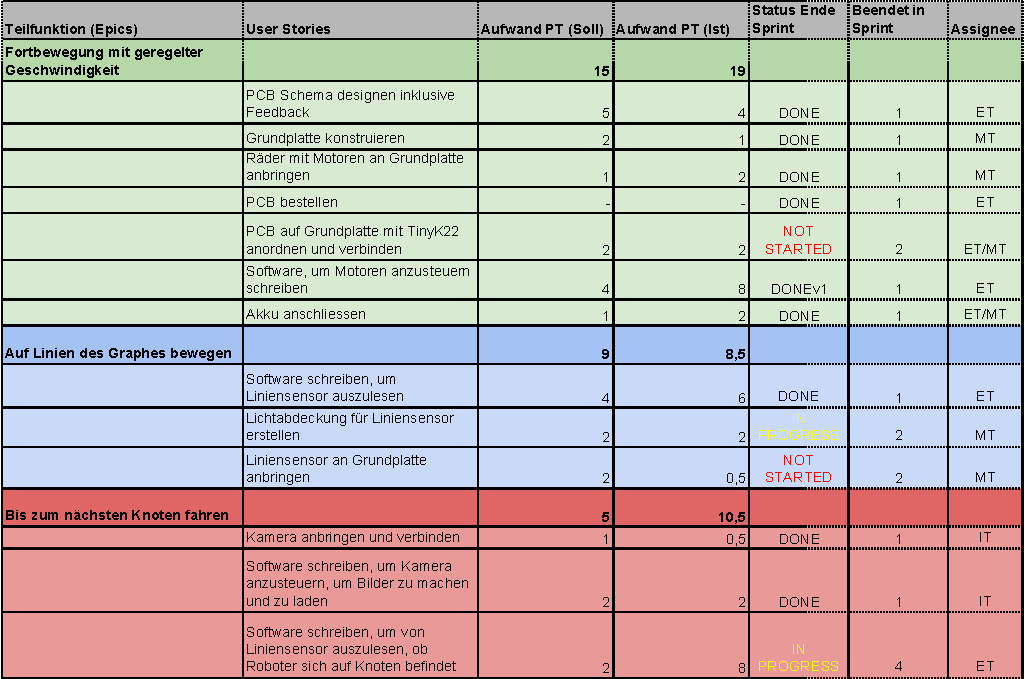
\includegraphics[width=\textwidth]{assets/projektmanagement/sprint1-crop.pdf}
\caption{Sprint 1 Backlog}
\label{table:sprint1-backlog}
\end{table}

Die Grundplatte des Roboters muss möglichst früh konstruiert werden, da diese existieren muss, damit die einzelnen Teile der drei geplanten Epics zusammengefügt werden können.


\textbf{Sprintreview}

Die Mehrheit der geplanten User Stories konnten umgesetzt werden.
Das \acrshort{pcb} wurde bestellt, ist jedoch noch nicht angekommen, weswegen Stories, die diese benötigen noch nicht begonnen oder fertig durchgeführt werden konnten.
Ebenfalls gab es eine Verzögerung bei dem Liniensensor. Die Software für den Liniensensor wurde bereits implementiert, ist aber noch nicht im Einsatz, da noch nicht alle Tests erfolgreich waren.

Folglich wurden zwei der drei definierten Sprintziele wie folgt erreicht:
\begin{itemize}
    \item Der Roboter kann von Software gesteuert geradeaus fahren.
    \item Der Roboter kann noch nicht von Software gesteuert einer Linie folgen oder mithilfe des Liniensensors einen Knoten erreichen.
    \item Der Roboter kann von einem Knoten zum Nachbarsknoten fahren, indem die Distanz gemessen wird, insofern der Knoten sich gerade vor dem Roboter befindet.
\end{itemize}


Es konnte bereits mit einigen Aufgaben von Sprint 2 begonnen werden:

\begin{itemize}
    \item Für den Epic 'Wegfindung' konnte bereits im ersten Sprint die Schnittstelle zwischen Steuerung und Navigation definiert werden. Ebenso konnte bereits die Software des Simulators angepasst werden, damit diese für die Navigation verwendet werden kann. Die Kommunikation zwischen Steuerung und Navigation konnte bereits begonnen werden.
    \item Für den Epic 'Hindernis umplatzieren' konnte bereits der Greifer an der Grundplatte angebracht werden.
\end{itemize}



\textbf{Risikoupdate}
\label{risks-sprint-1}

In diesem Sprint konnten folgende Risiken beseitigt oder minimiert werden:
\begin{itemize}
    \item Risiko 11: Kamera liefert unscharfe oder verzerrte Bilder: Kamera wurde intensiv verwendet und liefert sehr gute Bilder, insofern sie im Stillstand ist.
\end{itemize}

Es kam ein neues Risiko hinzu und wurde ebenfalls direkt minimiert:
\begin{itemize}
    \item Risiko 18: Akkuhalterung geht kaputt: Es wurden mehrere Akkuhalterungen gedruckt.
\end{itemize}


\newpage



\subsection{Sprint 2}

\textbf{Sprintziele:}
\begin{itemize}
    \item Die Navigation soll mit der Steuerung kommunizieren können.
    \item Der Roboter soll eine Kamera angeschlossen haben.
    \item Der Roboter soll von Software gesteuert ein Hindernis umplatzieren können.
    \item Der Roboter soll sich von Software gesteuert drehen können.
    \item Der Roboter soll sich von Software gesteuert in dem Winkel einer bestimmten ausgehenden Linie ausrichten können.
\end{itemize}

\textbf{Sprintbacklog:} Der Sprintbacklog von Sprint 2 ist in Tabelle 
% \ref{table:sprint2-backlog} 
dargestellt.

BILD KOMMT WENN PROJEKTCONTROLLING DURCHGEFUEHRT
% \begin{table}[H]
% \centering
% 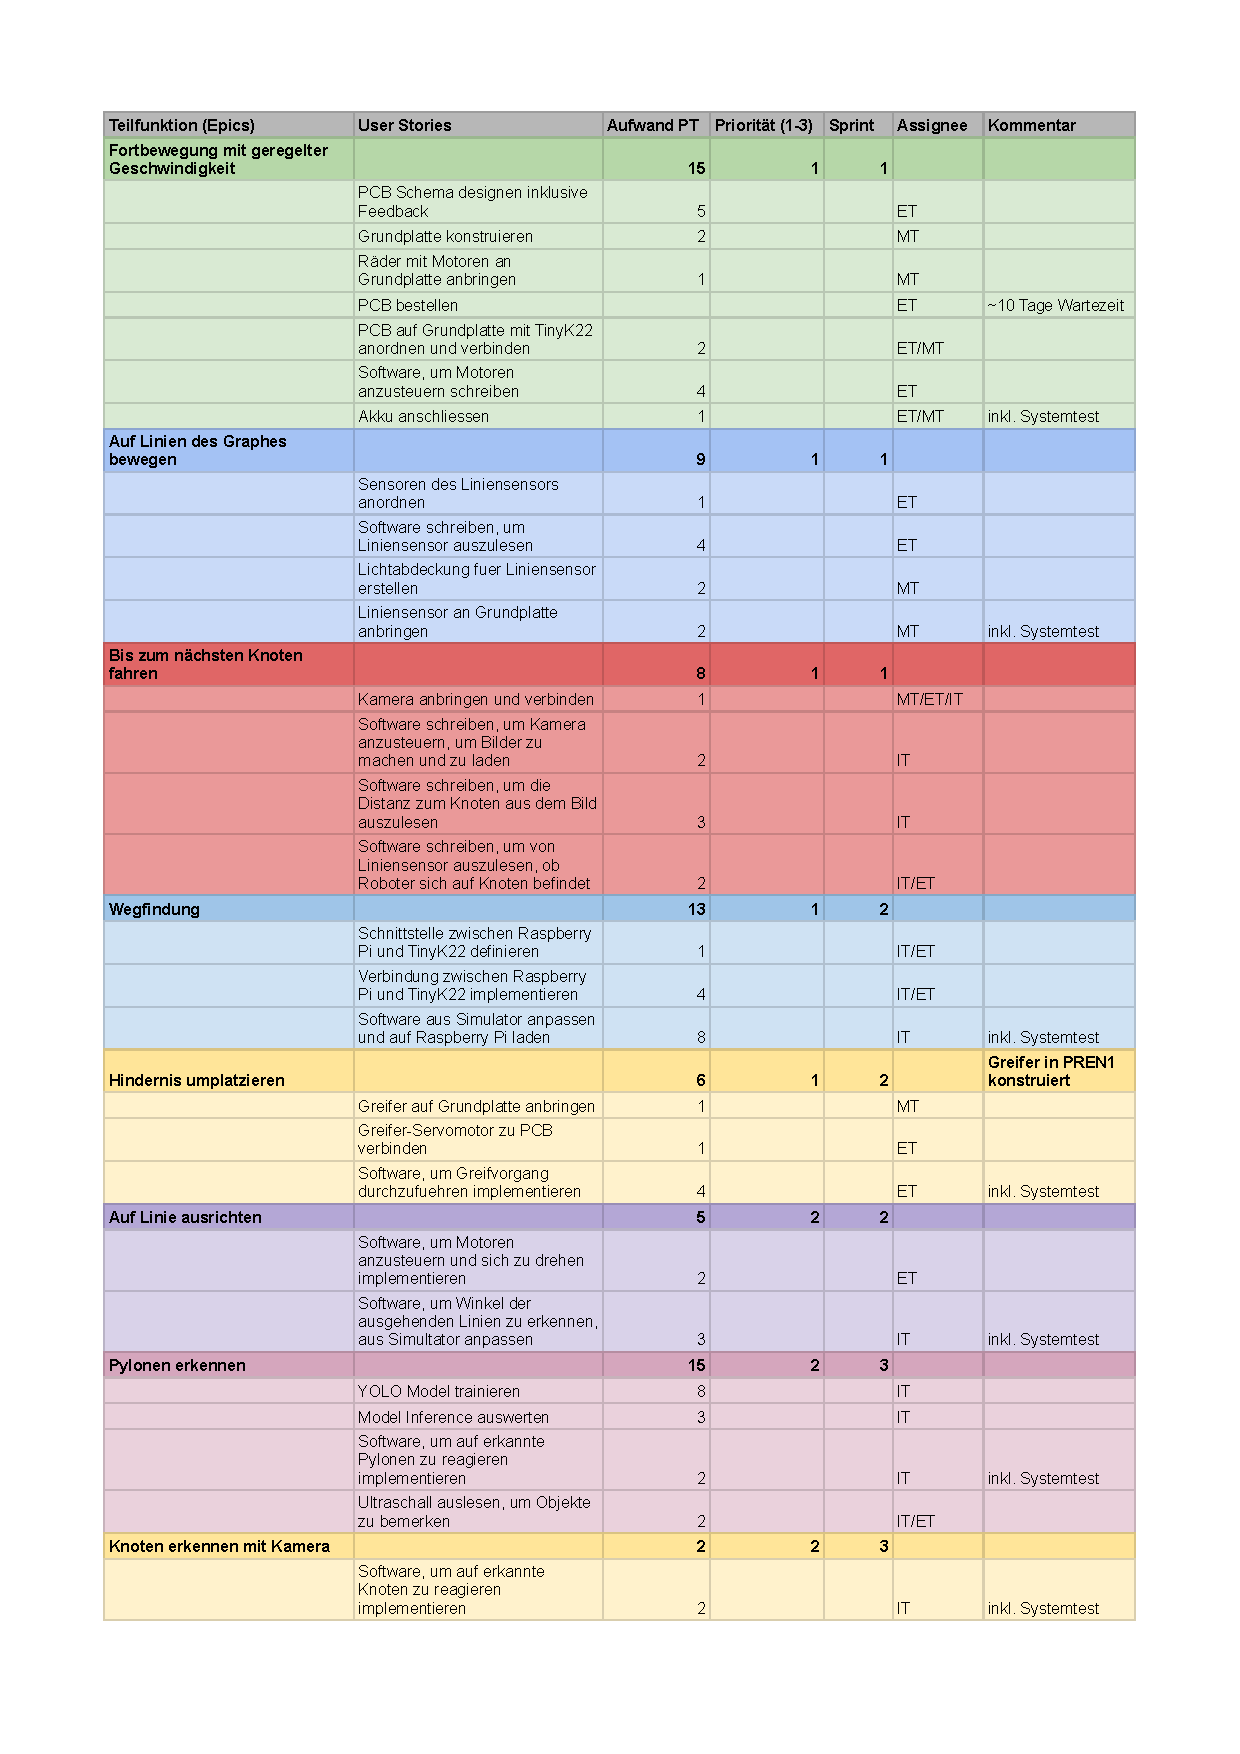
\includegraphics[width=\textwidth]{assets/projektmanagement/releaseplan-alle-sprints.pdf}
% \caption{Sprint 2 Backlog}
% \label{table:sprint2-backlog}
% \end{table}


\textbf{Sprintreview}

Mehrere Stories, die in Sprint 1 noch nicht umgesetzt werden konnten, konnten in Sprint 2 fertig gemacht werden: Das PCB ist angekommen und konnte auf der Grundplatte angebracht werden und mit dem TinyK22 und dem Liniensensor verbunden werden. Ebenfalls konnten die Lichtabdeckungen für den Liniensensor gefertigt und angebracht werden. Der Liniensenor selbst wurde ebenfalls fertiggestellt.

Im Sprint 2 konnten alle Stories des Wegfindungs Epics fertiggestellt werden: Schnittstelle wurde definiert und implementiert. Die Software des Simulators wurde bereits im Vorherigen Sprint angepasst.
Der Greifer ist seit Sprint 1 auf der Grundplatte angebracht und der Motor wurde an das PCB angeschlossen. Eine erste Version der Software dafür ist implementiert, jedoch wurde diese noch nicht getestet. Der Roboter kann die Winkel des ausgehenden Linien erkennen und sich drehen.

Es wurden drei der fünf definierten Sprintziele wie folgt erreicht:
\begin{itemize}
    \item Die Navigation kann über UART mit der Steuerung kommunizieren.
    \item Der Roboter hat eine Kamera angeschlossen und kann Bilder machen und speichern.
    \item Der Roboter kann noch nicht ein Hindernis von Software gesteuert heben.
    \item Der Roboter kann sich von Software gesteuert drehen. Er dreht sich aber noch nicht im korrekten Winkel.
    \item Der Roboter kann die ausgehenden Linien erkennen.
\end{itemize}

Ebenfalls konnten einige Stories aus nachfolgenden Sprints begonnen oder bereits beendet werden:
\begin{itemize}
    \item Der Epic 'Zieleingabe' aus Sprint 3 konnte umgesetzt werden.
    \item Für den Epic 'Ziel erreicht Ausgabe' aus Sprint 4 konnte bereits ein Buzzer angebracht werden, der von Software betätigt werden kann.
    \item Der Epic 'Not-Stop' aus Sprint 4 konnte bereits umgesetzt werden. Ein Schalter, der als Not-Stop dient, wurde angebracht und verbunden.
\end{itemize}


\textbf{Risikoupdate}
\label{risks-sprint-2}

In diesem Sprint konnten folgende Risiken beseitigt oder minimiert werden:
\begin{itemize}
    \item Risiko 13: Ein Softwarefehler führt zu einem Absturz: Dieses Risiko wird laufend miniemiert durch die Erstellung von Unittests.
    \item Risiko 14: Ein Software-Update fuehrt zu Fehlern: Jede neue Version wird getestet. Durch die Verwendung von Git kann die Software einfach auf eine alte Version zurückgesetzt werden.
    \item Risiko 4: 1 Minute reicht nicht zum Aufbau: Die Zieleingabe ist sehr simpel und schnell.
    \item Risiko xx:
\end{itemize}

Es kam ein neues Risiko hinzu und wurde ebenfalls direkt minimiert:
\begin{itemize}
    \item Risiko 19: Elektroteile gehen kaputt: Alle Elektroteile sind in mindestens zweifacher Ausgabe vorhanden. Das PCB ist fünf Mal vorhanden.
    \item ...
\end{itemize}
\newpage

\subsection{Sprint 3}

\textbf{Sprintziele:}
\begin{itemize}
    \item Der Roboter soll erkennen, ob sich eine Pylone vor ihm befindet.
    \item Der Roboter soll erkennen, ob sich eine Barriere vor ihm befindet.
    \item Der Roboter soll erkennen, ob eine erwartete Linie fehlt.
    \item Der Roboter soll erkennen, ob sich ein Knoten innerhalb von 2 Metern vor ihm befindet.
    \item Der Roboter soll selber erkennen, ob ein Knoten befahrbar ist oder ober er von einer Pylone blockiert ist.
    \item Der Roboter soll erkennen, ob eine Barriere auf der Linie vor ihm befindet und abwaegen, ob dieser Weg trotz Hindernisbeseitigung noch schnell genug ist.
    \item Der Roboter braucht eine Zieleingabe.

\end{itemize}

\textbf{Sprintbacklog:} Der Sprintbacklog von Sprint 3 ist in Tabelle 
% \ref{table:sprint3-backlog} 
dargestellt.

BILD KOMMT WENN PROJEKTCONTROLLING DURCHGEFUEHRT

% \begin{table}[H]
% \centering
% 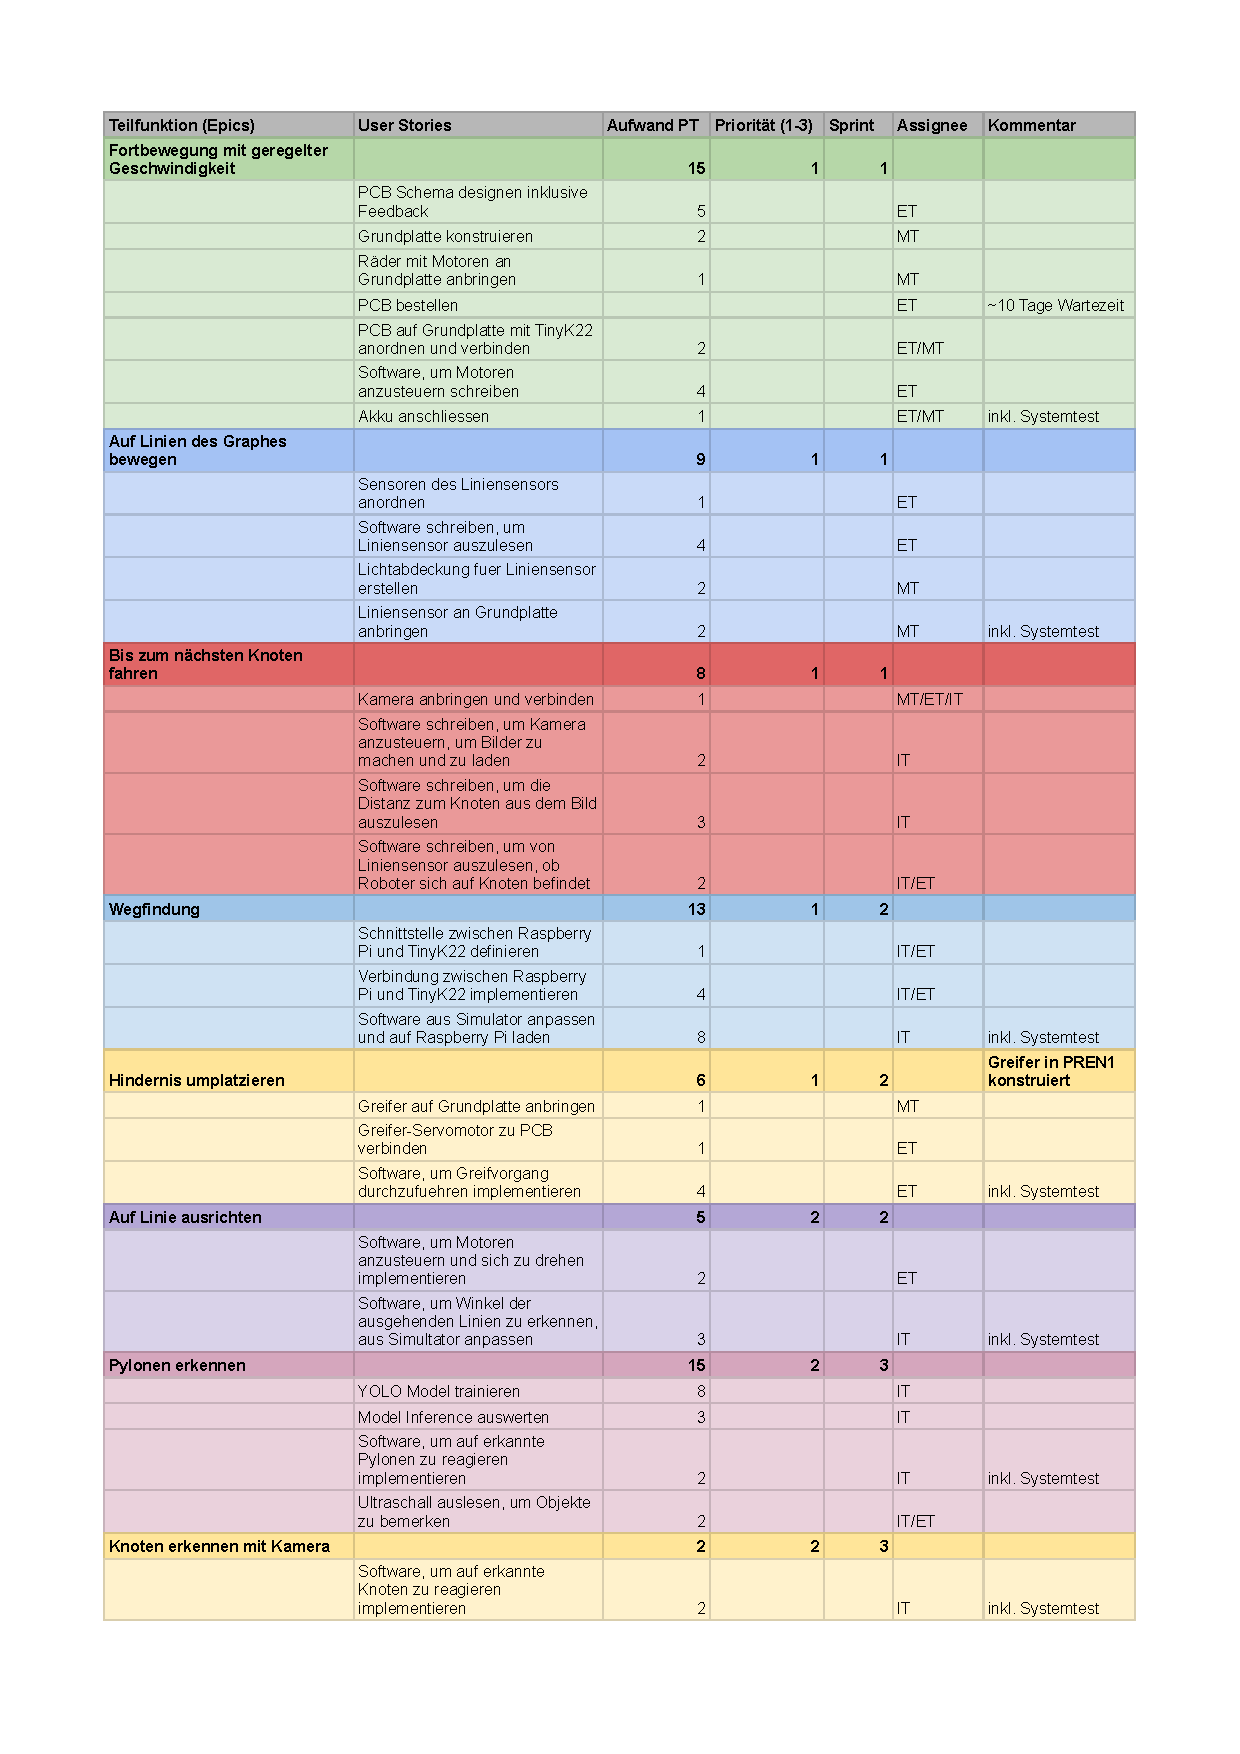
\includegraphics[width=\textwidth]{assets/projektmanagement/releaseplan-alle-sprints.pdf}
% \caption{Sprint 3 Backlog}
% \label{table:sprint3-backlog}
% \end{table}

Der Roboter muss bereits in der Lage sein sich durch einen Graphen zu bewegen, damit die Epics dieses Sprints integriert werden können.


\textbf{Sprintreview}

...

\textbf{Risikoupdate}

...


\newpage


\subsection{Sprint 4}

\textbf{Sprintziele:}
\begin{itemize}
    \item Der Roboter soll im Notfall gestoppt werden können.
    \item Der Roboter soll erkennen, wenn er sich im Ziel befindet.
    \item Der Roboter soll bekannt geben, dass er sich im Ziel befindet.
\end{itemize}

\textbf{Sprintbacklog:} Der Sprintbacklog von Sprint 4 ist in Tabelle 
% \ref{table:sprint4-backlog} 
dargestellt.

BILD KOMMT WENN PROJEKTCONTROLLING DURCHGEFUEHRT

% \begin{table}[H]
% \centering
% 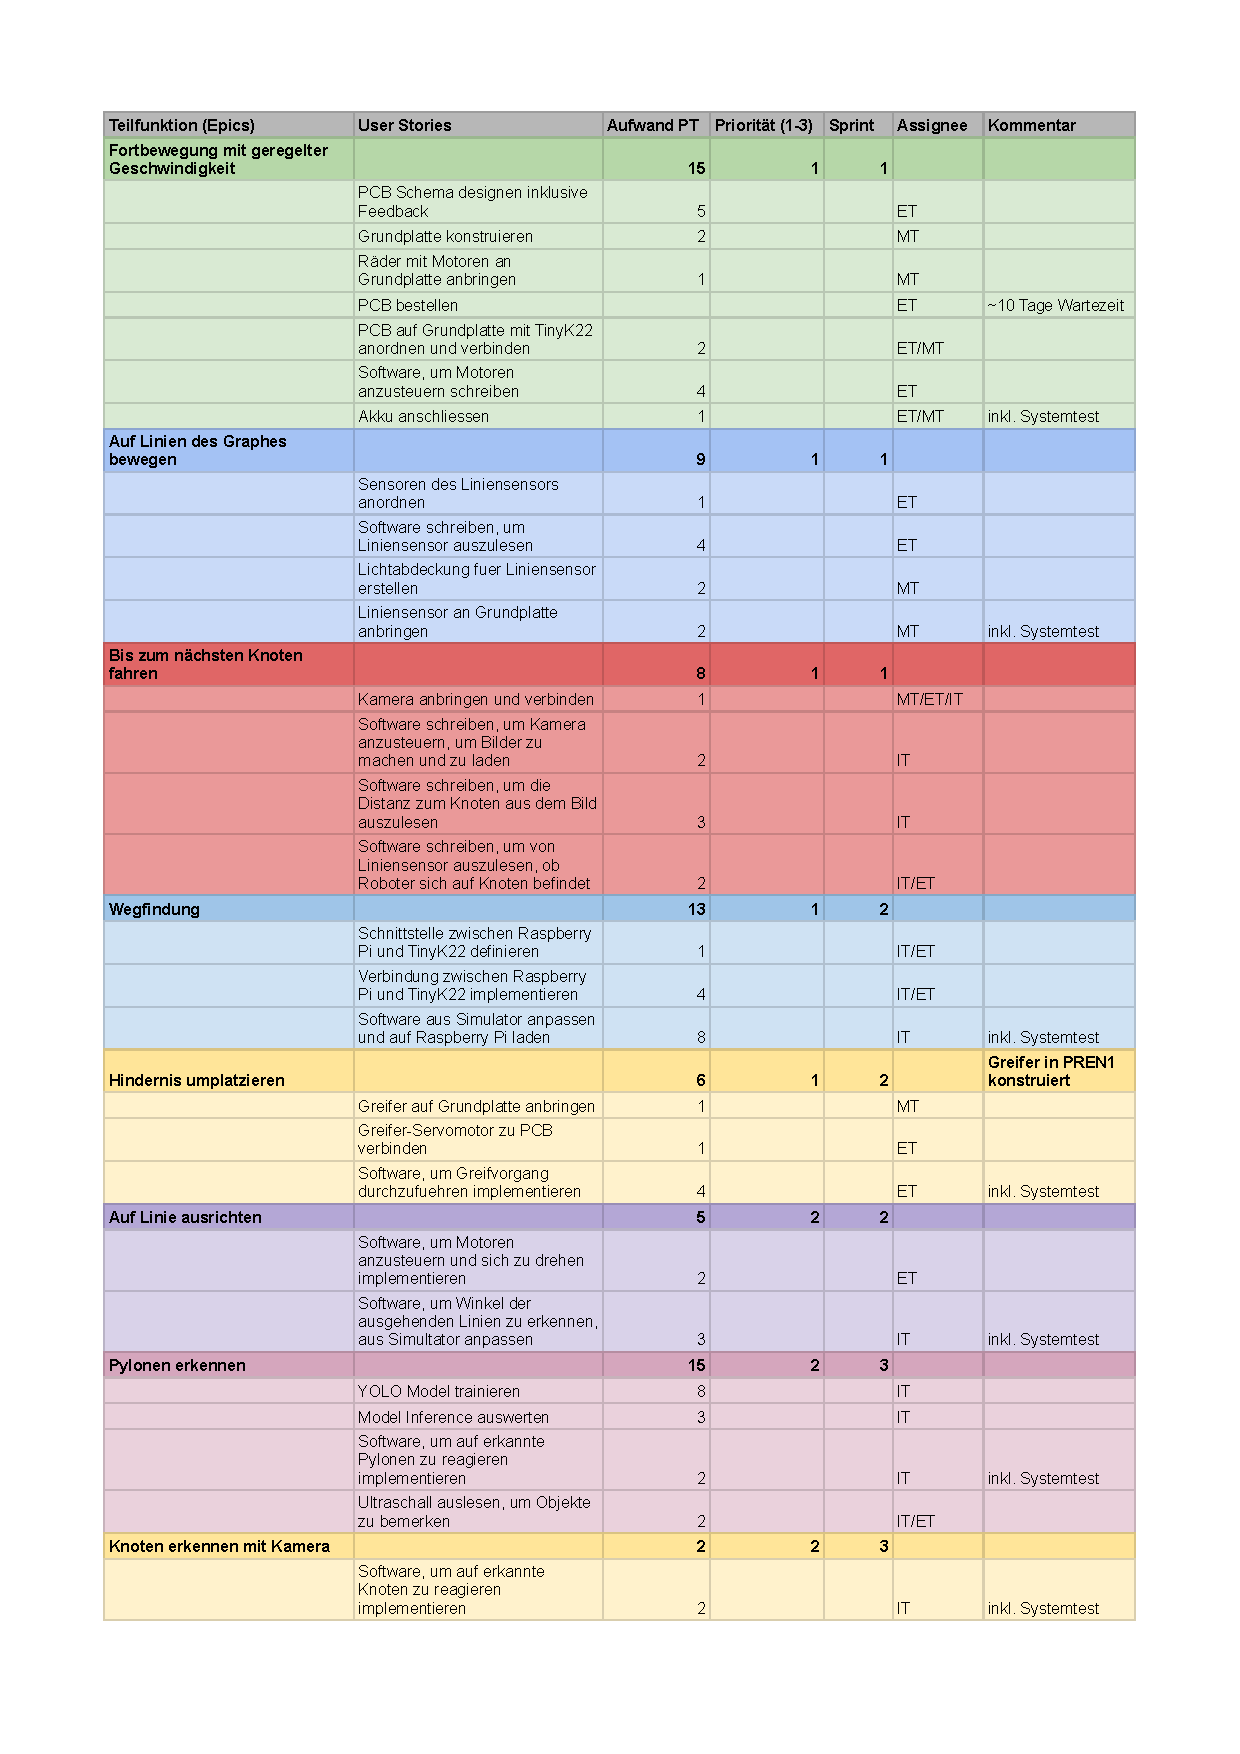
\includegraphics[width=\textwidth]{assets/projektmanagement/releaseplan-alle-sprints.pdf}
% \caption{Sprint 4 Backlog}
% \label{table:sprint4-backlog}
% \end{table}

Der Roboter soll bereits selbständig einen Graphen mit Hindernissen durchqueren können, damit die geplanten Epics umgesetzt werden können.


\textbf{Sprintreview}

...


(Folglich wurden zwei der drei definierten Sprintziele wie folgt erreicht:)
\begin{itemize}
    \item ...
    \item Der Roboter kann durch auslesen des Knoten vor sich erkenne, ob er sich im Ziel befindet.
    \item ...
\end{itemize}


\textbf{Risikoupdate}

...

\newpage